\documentclass{beamer}
\usepackage{amssymb,amsfonts,amsmath,graphicx,mathtools}
\usepackage{MnSymbol}
\title{Semisimple 2-categories}
\author{Ying Hong Tham}
\institute{UHH}
\date{2022}

\usepackage{tikz-cd}
%\usepackage{mystyle} % bad, beamer doesn't like newtheorem..

%% stuff from mystyle
\newcommand{\kk}{{\mathbf{k}}}
\newcommand{\ZZ}{{\mathbb{Z}}}
\newcommand{\ov}{\overline}
\newcommand{\del}{\partial}
\newcommand{\tnsr}{\otimes}
\newcommand{\vphi}{\varphi}
\newcommand{\veps}{{\varepsilon}}
\DeclareMathOperator{\Hom}{Hom} % \hom is already defnd
\DeclareMathOperator{\id}{id}
\DeclareMathOperator{\Obj}{Obj}
\DeclareMathOperator{\Rep}{Rep}
\newcommand{\inv}{{-1}} % annoying to type {-1} when taking inverse

\newtheorem{proposition}[theorem]{Proposition}

%%
\newcommand{\cB}{{\mathcal{B}}}
\newcommand{\cC}{{\mathcal{C}}}
\newcommand{\cD}{{\mathcal{D}}}
\newcommand{\cHom}{{\mathcal{H}\text{om}}}
\newcommand{\cFun}{{\mathcal{F}un}}
\newcommand{\Vect}{{\textrm{Vec}}}
\newcommand{\bigboxplus}{\Huge \boxplus}

\newcommand{\bimod}[2]{{#1\textrm{-bimod-}#2}}
\newcommand{\amod}[1]{{#1\textrm{-mod}}}
\newcommand{\moda}[1]{{\textrm{mod-}#1}}
\newcommand{\Mod}{{\mathcal{M}\textrm{od}}}
\newcommand{\ModA}[1]{{\Mod(#1)}}


\begin{document}

\frame{\titlepage}

%%%%%%%%%%%%%%%%%%%%%%%%%%%%%%%%%%%%%%%%%%%%%%%%%%%%%%%%%%%%%
\begin{frame}
\frametitle{Goal}
$\{\text{multifusion category}\}
\xrightarrow[\simeq]{\Mod_{s.s.}^{fin}(-)}
\{\text{finite semisimple 2-cat}\}$
\\

\begin{itemize}
\item The 2-category $\Mod_{s.s.}^{fin}(C)$
of finite semisimple module categories
over a multifusion category $C$
is semisimple.

\item For any finite semisimple 2-category $\cC$,
there exists a multifusion category $C$ such that
$\cC \simeq \Mod_{s.s.}^{fin}(C)$
\end{itemize}
\end{frame}

%%%%%%%%%%%%%%%%%%%%%%%%%%%%%%%%%%%%%%%%%%%%%%%%%%%%%%%%%%%%%
\begin{frame}
\frametitle{Conventions}
In relation to a 2-category:
\begin{itemize}
\item $\cC$ (caligraphic font): 2-category;

\item $X,Y,F$ (upper case latin): object of 2-category,
	functor between 2-categories;

\item $f,g$ (lower case latin): 1-morphism;
	we write $\cC(X,Y)$ for the category of morphisms
	from $X$ to $Y$;

\item $\eta,\veps,\delta$ (lower case greek): 2-morphism;
	for a 2-morphism $\alpha: f \Rightarrow g: X \to Y$,
	we may write $\alpha \in \cC(X,Y)(f,g)$
	to indicate its sources and targets,
	or simply $\alpha \in \Hom(f,g)$ if the objects are clear
\end{itemize}

\end{frame}


%%%%%%%%%%%%%%%%%%%%%%%%%%%%%%%%%%%%%%%%%%%%%%%%%%%%%%%%%%%%%
\begin{frame}
\frametitle{Conventions}
In relation to a 1-category:
\begin{itemize}
\item $C,A$ (upper case latin): category;

\item $a,b,f,g$ (lower case latin): objects in category,
	functor between categories;

\item $\alpha,\beta$ (lower case greek): morphism in category
\end{itemize}

\end{frame}


%%%%%%%%%%%%%%%%%%%%%%%%%%%%%%%%%%%%%%%%%%%%%%%%%%%%%%%%%%%%%
\begin{frame}
\frametitle{Conventions}
We also compose morphisms from right to left:
in a 2-category $\cC$,
for $\alpha \in \cC(X,Y)(f,f'),
\beta \in \cC(Y,Z)(g,g'),
\gamma \in \cC(X,Y)(f',f'')$,
we write:

for composition of 1-morphisms,
\[
g \circ f, g \circ f', \ldots : X \to Z
\]
for horizontal composition of 2-morphisms,
\[
\beta \circ \alpha: (g \circ f) \Rightarrow (g' \circ f'):
	X \to Z
\]
for vertical composition of 2-morphisms,
\[
\gamma \cdot \alpha: f \Rightarrow f'' : X \to Y
\]

\end{frame}


%%%%%%%%%%%%%%%%%%%%%%%%%%%%%%%%%%%%%%%%%%%%%%%%%%%%%%%%%%%%%
\begin{frame}
\frametitle{Conventions}
In general, if $P$ is a property of a 1-category,
we say that a 2-category $\cC$ is \emph{locally $P$}
if every hom-category $\cC(X,Y)$ satisfies $P$.

\pause

By 2-category we always mean a weak 2-category
that is furthermore locally additive over $\kk$.

By 2-functor (sometimes just functor for simplicity)
between 2-categories will always be locally $\kk$-linear.

\end{frame}

%%%%%%%%%%%%%%%%%%%%%%%%%%%%%%%%%%%%%%%%%%%%%%%%%%%%%%%%%%%%%
\begin{frame}

\begin{center}
\Huge Review
\end{center}
\end{frame}

%%%%%%%%%%%%%%%%%%%%%%%%%%%%%%%%%%%%%%%%%%%%%%%%%%%%%%%%%%%%%
\begin{frame}
\frametitle{Additive 2-category, direct sum of objects}

\pause

\begin{definition}[direct sum of objects in 2-category]
A \emph{direct sum} of two objects $A_1,A_2$ in $\cC$
is an object $A_1 \boxplus A_2$ together with
inclusion and projection 1-morphisms
$i_k : A_k \rightleftharpoons A_1 \boxplus A_2 : p_k$,
such that
\begin{itemize}
\item $p_k \circ i_k \simeq \id_{A_k}$,
\item $p_2 \circ i_1$, $p_1 \circ i_2$ are zero 1-morphisms,
\item $\id_{A_1 \boxplus A_2} \simeq
	i_1 \circ p_1 \oplus i_2 \circ p_2$
\end{itemize}
\end{definition}

\pause

\begin{definition}[zero object]
A \emph{zero object} in $\cC$
is an object $0$ with trivial endomorphism category
$\cC(0,0)$ (has one object $\id_0$
with only identity morphism $\id_{\id_0}$.
\end{definition}

\pause

\begin{definition}
2-category $\cC$ is \emph{additive}
if finite direct sums of objects exist,
has a zero object,
(and is locally additive).
\end{definition}


\end{frame}


%%%%%%%%%%%%%%%%%%%%%%%%%%%%%%%%%%%%%%%%%%%%%%%%%%%%%%%%%%%%%
\begin{frame}
\frametitle{Additive 2-category, direct sum of objects}

\begin{proposition}
$i_k,p_k$ are two-sided adjoints to each other.
\end{proposition}

\pause

\begin{definition}
A 1-morphism $i: X \to Y$ is \emph{fully faithful}
(or $(X,i)$ is a \emph{subobject} of $Y$)
if it induces fully faithful functors between hom-categories
by post-composition, i.e. for all objects $A$,
$i \circ - : \cC(A,X) \to \cC(A,Y)$
is fully faithful.
\end{definition}

\pause

\begin{proposition}
$i_k: A_k \to A_1 \boxplus A_2$ is fully faithful.
\end{proposition}


\end{frame}
%%%%%%%%%%%%%%%%%%%%%%%%%%%%%%%%%%%%%%%%%%%%%%%%%%%%%%%%%%%%%
\begin{frame}
\frametitle{Additive 2-category, direct sum of objects}

\begin{definition}[Direct sum of 2-categories]
Given 2-categories $\cC_j$, $j \in J$,
we may consider the direct sum 2-category
$\cC := \bigboxplus_{j \in J} \cC_j$:
\begin{itemize}
\item $\Obj \cC = \prod_{j \in J} \Obj \cC_j$

\pause

\item for $X_i \in \cC_i, Y_j \in \cC_j$,
	$\cC(X_i,Y_j) =
\begin{cases}
	\cC_j(X_i,Y_j) \;\; \text{if } i = j
	\\
	0 \;\; \text{if } i \neq j
\end{cases}
$

\pause

\item extend by direct sums:
	$\cC(\boxplus X_i, \boxplus Y_j)
	= \bigoplus \cC_i(X_i, Y_i)$
\end{itemize}
\end{definition}

\end{frame}

%%%%%%%%%%%%%%%%%%%%%%%%%%%%%%%%%%%%%%%%%%%%%%%%%%%%%%%%%%%%%
\begin{frame}
\frametitle{Idempotent completeness, separable monads, splittings}

\pause

\begin{definition}
A \emph{separable algebra} $(a,\mu,\eta)$ in a tensor category $C$
is an algebra that admits an $a$-$a$-bimodule section
$\prescript{}{a}a_a \to \prescript{}{a}a \tnsr a_a$
to $\mu$.
\end{definition}

\pause

\begin{definition}
Let $(t, \mu, \eta)$ be a monad on an object $X$
in a 2-category $\cC$.
We say $t$ is \emph{separable} if there is a
$t$-$t$-bimodule section
$t \Rightarrow t \circ t$ to $\mu$.
\end{definition}

\pause

In other words, a separable monad over $X$
is a separable algebra in $\cC(X,X)$.

\end{frame}

%%%%%%%%%%%%%%%%%%%%%%%%%%%%%%%%%%%%%%%%%%%%%%%%%%%%%%%%%%%%%
\begin{frame}
\frametitle{Idempotent completeness, separable monads, splittings}

\begin{definition}
Let $r \vdash l: X \to Y$ be an adjunction
with unit $\eta: \id_X \Rightarrow rl$
and counit $\veps: lr \Rightarrow \id_Y$.
We say the adjunction $l \dashv r$ is \emph{separable}
if $\veps$ admits a section.
\end{definition}

\pause

Clearly, if an adjunction $l \dashv r$ is separable,
then the monad $rl$ is separable.

\pause

\begin{definition}
Let $(t,\mu,\eta)$ be a separable monad on
an object $X \in \cC$.
A \emph{(separable) splitting} of $t$ is a (separable) adjunction
$r \vdash l: X \to Y$
together with an isomorphism
$\psi: rl \simeq t$ as monads on $X$.
\end{definition}

\pause

Under the right conditions
(local idempotent completeness of $\cC$),
splittings are unique:

\begin{proposition}[Uniqueness of splitting]
[\cite{DRfusion}, Theorem A.3.1]
\label{p:splitting-unique}
In a locally idempotent complete 2-category $\cC$,
splittings of a separable monad are unique
up to equivalence.
\end{proposition}

%In particular, this holds true when $\cC$
%is locally semisimple.

\end{frame}

%%%%%%%%%%%%%%%%%%%%%%%%%%%%%%%%%%%%%%%%%%%%%%%%%%%%%%%%%%%%%
\begin{frame}
\frametitle{Idempotent completeness, 2-category}

\begin{definition}
A 2-category $\cC$ is \emph{idempotent complete}
if every separable monad admits a splitting
and is locally idempotent complete.
\end{definition}

\pause

\begin{definition}[Idempotent completion]
Let $\cC$ be a locally idempotent complete 2-category.
The \emph{idempotent completion of $\cC$},
denoted $\cC^\nabla$, with:
\begin{itemize}
\item Objects: $(X,p)$ separable monad in $\cC$,
\item $\cC^\nabla((X,p),(Y,q)) = \bimod{q}{p}(\cC(X,Y))$
\end{itemize}

\pause

There is a natural 2-functor $I: \cC \to \cC^\nabla$
that is fully faithful.

\pause

A 2-functor $F: \cC \to \cD$
extends to a 2-functor $F^\nabla: \cC^\nabla \to \cD^\nabla$
that commutes with $I$'s.
\end{definition}

\end{frame}

%%%%%%%%%%%%%%%%%%%%%%%%%%%%%%%%%%%%%%%%%%%%%%%%%%%%%%%%%%%%
\begin{frame}
\frametitle{Idempotent completeness, 2-category}

Key example:

$\cB C$: one object $*$ with endomorphism category
$\cB C(*,*)$.

\[
(\cB C)^\nabla =
\begin{cases}
	\Obj: \text{ separable algebras in } C
	\\
	\text{Mor}: (\cB C)^\nabla (a,b) = \bimod{b}{a}(C)
\end{cases}
\]


\end{frame}

%%%%%%%%%%%%%%%%%%%%%%%%%%%%%%%%%%%%%%%%%%%%%%%%%%%%%%%%%%%%%
\begin{frame}
\frametitle{Idempotent completeness, 2-category}

\begin{proposition}
$\cC^\nabla$ is idempotent complete.
Moreover, if $\cC$ is already idempotent complete,
then $I: \cC \simeq \cC^\nabla$ is an equivalence.
\end{proposition}

\pause

As a consequence, if $\cD$ is idempotent complete,
then we have equivalences of 2-categories
\[
\cFun(\cC,\cD) \simeq \cFun(\cC^\nabla,\cD^\nabla)
\simeq \cFun(\cC^\nabla, \cD)
\]

\pause

\begin{proposition}
If $F: \cC \to \cD$ is fully faithful,
then $F^\nabla: \cC^\nabla \to \cD^\nabla$
is also fully faithful.
\end{proposition}

\end{frame}

%%%%%%%%%%%%%%%%%%%%%%%%%%%%%%%%%%%%%%%%%%%%%%%%%%%%%%%%%%%%
\begin{frame}
\frametitle{Idempotent completeness, 2-category}


\begin{proposition}[\cite{DRfusion}{Prop 1.3.13}]
\label{p:modC-deloop}
For a multifusion category $C$,
the following 2-functor is an equivalence:
\begin{align*}
\amod{(-)}(C): (\cB C)^\nabla
	& \to
	\ModA{C}
\\
a & \mapsto
	\amod{a}(C)
\\
\prescript{}{b}m_a & \mapsto
	m \tnsr_a -
\\
\vphi & \mapsto
\vphi \tnsr_a -
\end{align*}
\end{proposition}

\end{frame}

%%%%%%%%%%%%%%%%%%%%%%%%%%%%%%%%%%%%%%%%%%%%%%%%%%%%%%%%%%%%
\begin{frame}
\frametitle{Idempotent completeness, 2-category}

\begin{proof}
Essential surjectivity follows from:\\
-\cite{Ostrik}{Theorem 1}: for a finite semisimple right module
category over multifusion $C$, there exists a semisimple algebra
$a$ in $C$ such that $M \simeq \amod{a}(C)$
as right $C$-module categories; and

\pause
-\cite{DSPSb}{Corollary 2.6.9}: When $C$ is multifusion over
a field of characterisitc 0,
a right $C$-module category $M$ is separable
($\simeq \amod{a}(C)$ for a separable algebra $a$)
if and only if it is semisimple.

\pause

Fully faithfulness follows from \cite{EGNO}{Prop 7.11.1}.
\end{proof}

\pause

This is almost one half of the main result;
one still needs to prove local semisimplicity
and existence of adjoints.
This will follow from more results from \cite{DSPSa},\cite{DSPSb},
which we show later.

\end{frame}
%%%%%%%%%%%%%%%%%%%%%%%%%%%%%%%%%%%%%%%%%%%%%%%%%%%%%%%%%%%%
\begin{frame}
\frametitle{Simple objects}

\pause

\begin{proposition}[equivalent notions of simple-ness]
Let $\cC$ be a locally finite semisimple and
idempotent complete 2-category,
and let $X \in \cC$ be a nonzero object.
Then the following notions of $X$ being simple are equivalent:

\pause

(1) any subobject $i: Y \to X$ of $X$
 is either 0 or an equivalence;

\pause

(2) $X$ cannot be written as a non-trivial direct sum,
	i.e. if $X = \boxplus X_i$,
	then $X_i \simeq 0$ for all but one $i$;

\pause

(3) $\id_X$ is a simple object in $\cC(X,X)$.
\end{proposition}

\end{frame}

%%%%%%%%%%%%%%%%%%%%%%%%%%%%%%%%%%%%%%%%%%%%%%%%%%%%%%%%%%%%
\begin{frame}
\frametitle{Simple objects}

\begin{proof}[Proof sketch]
(1) $\Rightarrow$ (2): Contravariant statement
follows from fully faithfulness of
$i_k: A_k \to A_1 \boxplus A_2$.

\pause

(2) $\Rightarrow$ (3): Contravariant statement is
``identity splitting implies object splitting'',
uses idempotent completeness of $\cC$
to split out objects corresponding to summands of $\id_X$
(which are separable monads)
(see \cite{DRfusion}{Prop 1.3.16}).

\pause

(3) $\Rightarrow$ (1): for non-zero fully faithful $r: Y \to X$,
with $\id_X$ simple,
consider the left adjoint $l: X \to Y$,
use fully faithfulness to get a preimage
$\delta : \id_Y \Rightarrow lr$ of
$\eta \circ r: r \Rightarrow rlr$.
%Use simplicity of $\id_X$ to get section of the unit $\eta$.
Show $\delta$ is a section of the counit. Etc.
(See \cite{DRfusion}{Prop 1.2.14})
\end{proof}

\end{frame}

%%%%%%%%%%%%%%%%%%%%%%%%%%%%%%%%%%%%%%%%%%%%%%%%%%%%%%%%%%%%%
\begin{frame}
\frametitle{Semisimple 2-category}

\begin{definition}[(finite) semisimple 2-category]

\pause

A 2-category $\cC$ is \emph{semisimple}
if it is:
\begin{itemize}
\item locally semisimple,
\item admits left and right adjoints for every 1-morphism,
\item additive,
\item idempotent complete.
\end{itemize}

It is furthermore \emph{finite semisimple}
if it is also locally finite and
has finitely many equivalence classes of simple objects.
\end{definition}

\end{frame}


%%%%%%%%%%%%%%%%%%%%%%%%%%%%%%%%%%%%%%%%%%%%%%%%%%%%%%%%%%%%%
\begin{frame}

\begin{center}
\Huge New Stuff
\end{center}

\end{frame}


%%%%%%%%%%%%%%%%%%%%%%%%%%%%%%%%%%%%%%%%%%%%%%%%%%%%%%%%%%%%%
\begin{frame}
\frametitle{Schur's lemma}

The equivalence between notions of a simple object
in a semisimple 2-category,
is similar to the semisimple 1-category case.

\pause

However, recall $\ModA{\Vect_{\ZZ/2}}$:

\[
\begin{tikzpicture}
\node (a) at (0,0) {$\Vect_{\ZZ/2}$};
\node (b) at (4,0) {$\Vect$};
\draw[->] (a) to[out=30,in=150] (b);
\node at (2,1) {\footnotesize $\Vect$};
\draw[->] (b) to[out=-150,in=-30] (a);
\node at (2,-1) {\footnotesize $\Vect$};
\draw[->] (a) .. controls +(-150:2cm) and +(150:2cm) .. (a);
\node at (-2,0) {\footnotesize $\Vect_{\ZZ/2}$};
\draw[->] (b) .. controls +(30:2cm) and +(-30:2cm) .. (b);
\node at (6,0) {\footnotesize $\Vect_{\ZZ/2}$};
\end{tikzpicture}
\]

\pause

There can be nonzero morphisms between
non-equivalent simple objects - weird!

\pause

``2-Morita equivalences'' between fusion categories


\end{frame}

%%%%%%%%%%%%%%%%%%%%%%%%%%%%%%%%%%%%%%%%%%%%%%%%%%%%%%%%%%%%%
\begin{frame}
\frametitle{Schur's lemma}

\begin{proposition}
[Schur's Lemma, \cite{DRfusion}{Prop 1.2.19}]
\label{p:schur-lemma}
In a semisimple 2-category $\cC$,
if $f: A \to B, g: B \to C$ are nonzero 1-morphisms
between simple objects $A,B,C$,
then $g \circ f$ is also nonzero.
\end{proposition}

\pause

\begin{proof}

\begin{tikzpicture}
\node (a) at (0,0) {$A$};
\node (b) at (2,0) {$B$};
\node (c) at (4,0) {$C$};
\draw[->] (b) -- (c) node[pos=0.5,above] {$g$};
\draw[->] (a) .. controls +(45:1cm) and +(135:1cm) .. (b)
	node[pos=0.5,above] {$f$};
\pause %%%%%%%%%%%%%%%%%%%%%%%
\draw[->] (b) .. controls +(-135:1cm) and +(-45:1cm) .. (a)
	node[pos=0.5,below] {$f^*$};
\draw[->] (b) .. controls +(-150:1cm) and +(150:1cm) .. (b);
\draw[-{Implies},double] (0.35,0.05) -- (1.2,0.05)
	node[pos=0.5,above] {\scriptsize $\veps$};
\pause %%%%%%%%%%%%%%%%%%%%%%%
\draw[-{Implies},double] (1.15,-0.05) -- (0.3,-0.05)
	node[pos=0.5,below] {\scriptsize $\exists \delta$};
\pause %%%%%%%%%%%%%%%%%%%%%%%
\node at (6,-1) {
	$\id_g = (\id_g \circ \veps) \cdot (\id_g \circ \delta):
g \Rightarrow gff^* \Rightarrow g$};
\end{tikzpicture}

\pause
Let $f^*: B \to A$ be a right adjoint to $f$.
%\pause
Since $\id_B$ is simple, $\exists$ section
$\delta: \id_B \Rightarrow ff^*$
to counit $\veps: ff^* \Rightarrow \id_B$.
%\pause
Postcomposing with $g$,
we have $\id_g = (\id_g \circ \veps) \cdot (\id_g \circ \delta):
g \Rightarrow gff^* \Rightarrow g$.
%\pause
Thus if $gf = 0$, then $\id_g = 0$,
contradicting nonzero-ness of $g$.
\end{proof}

\end{frame}

%%%%%%%%%%%%%%%%%%%%%%%%%%%%%%%%%%%%%%%%%%%%%%%%%%%%%%%%%%%%%
\begin{frame}
\frametitle{Schur's lemma - components}


\begin{definition}[component of semisimple 2-category]
In a semisimple 2-category $\cC$,
we say two simple objects $A,B$ belong to the same
\emph{component} if there exists a nonzero 1-morphism
$f: A \to B$.
\end{definition}

\pause

-transitivity from Schur's lemma, symmetry from adjoints,
reflexivity from identity

\pause

In a finite semisimple 2-category $\cC$,
there will be finite set $J$ of components;

\pause

full subcategory $\cC_j$, $j \in J$:
direct sum of simple objects in $j$

\pause

gives direct sum decomposition
$\cC \simeq \bigboxplus_{j \in J} \cC_j$.

\end{frame}


%%%%%%%%%%%%%%%%%%%%%%%%%%%%%%%%%%%%%%%%%%%%%%%%%%%%%%%%%%%%%
\begin{frame}
\frametitle{Main results}

\begin{theorem}[\cite{DRfusion}{Theorem 1.4.8}]
The 2-category of finite semisimple module categories
of a multifusion category $C$
is a finite semisimple 2-category.
\end{theorem}

\pause

\begin{proof}
$\ModA{C} \simeq (\cB C)^\nabla$ is idempotent complete
and locally idempotent complete.
$\ModA{C}$ is clearly already additive.


Locally semisimple-ness follows directly from
\cite{DSPSb}{Corollary 2.5.6},
and existence of adjoints for 1-morphisms
follows from \cite{DSPSa}{Corollary 2.13}.

\end{proof}

\end{frame}


%%%%%%%%%%%%%%%%%%%%%%%%%%%%%%%%%%%%%%%%%%%%%%%%%%%%%%%%%%%%%
\begin{frame}
\frametitle{Main results}

\begin{theorem}[\cite{DRfusion}{Theorem 1.4.9}]
Every finite semisimple 2-category is equivalent to
the 2-category of finite semisimple module categories
of a multifusion category.
\end{theorem}

\begin{proof}\renewcommand{\qedsymbol}{}
Assume that $\cC$ has only one component.

\pause
($\cC \simeq \bigboxplus_{j \in J} \cC_j$
and $\cC_j \simeq \ModA{C_j}$ for multifusion $C_j$,
then $\cC \simeq \ModA{\bigoplus_{j \in J} C_j}$.)

\pause
Fix simple object $X$, let $C = \cC(X,X)$.
\pause
%Since $\id_X$ is simple, $C$ is in fact fusion.

We show $\cC \simeq (\cB C)^\nabla$.

\end{proof}

\end{frame}

%%%%%%%%%%%%%%%%%%%%%%%%%%%%%%%%%%%%%%%%%%%%%%%%%%%%%%%%%%%%%
\begin{frame}
\frametitle{Main results}

\begin{proof}[Proof (Cont.)]\renewcommand{\qedsymbol}{}

Consider the inclusion 2-functor
\begin{align*}
F : \cB C &\to \cC
\\
* &\mapsto X
\end{align*}
which is fully faithful by construction.
\pause
Then
\[
F^\nabla: (\cB C)^\nabla \to \cC
\]
is fully faithful.
\pause
Remains to show other simples are in essential image.

\end{proof}

\end{frame}

%%%%%%%%%%%%%%%%%%%%%%%%%%%%%%%%%%%%%%%%%%%%%%%%%%%%%%%%%%%%%
\begin{frame}
\frametitle{Main results}

\begin{proof}[Proof (Cont.)]\renewcommand{\qedsymbol}{}

\begin{tikzpicture}
\node (st) at (0,0) {$*$};
\node (x) at (4,0) {$X$};
\node (y) at (5,2) {$Y$};
\draw[|->] (st) -- (x) node[pos=0.5,above] {$F^\nabla$};
\pause %%%%%%%%%%%%%%%%%%%%%%%%%
\draw[->] (x) to[out=80,in=-130] (y);
\node at (4.1,1) {$f$};
\pause %%%%%%%%%%%%%%%%%%%%%%%%%
\draw[->] (y) to[out=-100,in=50] (x);
\node at (4.9,1) {$g$};
\node at (4.5,1) {$\dashv$};
\pause %%%%%%%%%%%%%%%%%%%%%%%%%
\draw[->] (st) .. controls +(80:0.8cm) and +(40:0.8cm) .. (st);
\node at (0.7,0.7) {$gf$};
\pause %%%%%%%%%%%%%%%%%%%%%%%%%
\node (a) at (-1,2) {$(*,gf)$};
\draw[->] (st) to[out=130,in=-80] (a);
\draw[->] (a) to[out=-50,in=100] (st);
\pause %%%%%%%%%%%%%%%%%%%%%%%%%
\node (b) at (3,2) {$F^\nabla(*,gf)$};
\draw[->] (x) to[out=130,in=-80] (b);
\draw[->] (b) to[out=-50,in=100] (x);
\draw[|->] (a) -- (b) node[pos=0.5,above] {$F^\nabla$};
\pause %%%%%%%%%%%%%%%%%%%%%%%%%
\draw[->] (b) -- (y) node[pos=0.5,above] {$\simeq$};
\end{tikzpicture}

\pause
Simple object $Y$,
%\pause
$\exists$ nonzero 1-morphism $f: X \to Y$;
%\pause
has (nonzero) right adjoint $g: Y \to X$,
with counit $\veps : fg \Rightarrow \id_Y$.
%\pause
$\id_Y$ is simple, so $\veps$ admits a section,
%\pause
hence $f \dashv g$ is a separable adjunction.
%\pause
Thus, by uniqueness of separable splittings,
$Y$ is in the essential image of $F^\nabla$.

\end{proof}

\end{frame}

%%%%%%%%%%%%%%%%%%%%%%%%%%%%%%%%%%%%%%%%%%%%%%%%%%%%%%%%%%%%%
\begin{frame}
\frametitle{Main results}


The only property of $X$ that we used is the fact that
there exists a nonzero 1-morphism from $X$ to every simple
in $\cC$,
and thus any nonzero $X$ will do.
\pause
Taking, say, $X = \boxplus X_i$,
where the sum is over equivalence classes of simples,
would result in a multifusion $C = \cC(X,X)$.

\pause
We can also avoid the first step of taking only one component
of $\cC$,
take $X$ with at least one object from each $\cC_j$
in its direct sum decomposition.

\end{frame}

%%%%%%%%%%%%%%%%%%%%%%%%%%%%%%%%%%%%%%%%%%%%%%%%%%%%%%%%%%%%%
\begin{frame}
\frametitle{Main results}

Every object contains within them
the data to reconstruct the whole 2-category.

\begin{tikzpicture}
\draw (0.9,0.5) circle (2.5cm);
\node (x) at (0,0) {$X$};
\node (y) at (2,0) {$Y$};
\node (z) at (1,1.5) {$\amod{a}(C)$};
%%
\draw[->] (x) .. controls +(-120:1cm) and +(180:1cm) .. (x);
\draw[->] (y) .. controls +(0:1cm) and +(-60:1cm) .. (y);
\draw[->] (z) .. controls +(120:1cm) and +(60:1cm) .. (z);
\node at (-0.2,-0.8) {$C \ni a$};
%
\draw[->] (x) .. controls +(20:0.8cm) and +(160:0.8cm) .. (y);
\draw[->] (z) .. controls +(-100:0.8cm) and +(40:0.8cm) .. (x);
%
\draw[->] (y) .. controls +(-160:0.8cm) and +(-20:0.8cm) .. (x);
\draw[->] (z) -- (y)
	node[pos=0.5,right] {$\simeq$};
\draw[->] (x) .. controls +(80:0.8cm) and +(-140:0.8cm) .. (z);
%%%%%%%%%%%%%%%%%%%%%%%%%%%%%
\begin{scope}[shift={(5,0.5)}]
\draw (1,0) circle (2cm);
\node (a) at (0,0) {$A$};
\node (b) at (2,0) {$B$};
%%
\draw[->] (a) .. controls +(-150:1cm) and +(150:1cm) .. (a);
\draw[->] (b) .. controls +(30:1cm) and +(-30:1cm) .. (b);
%
\draw[->] (a) .. controls +(20:0.8cm) and +(160:0.8cm) .. (b);
\draw[->] (b) .. controls +(-160:0.8cm) and +(-20:0.8cm) .. (a);
\end{scope}
\end{tikzpicture}

\end{frame}

%%%%%%%%%%%%%%%%%%%%%%%%%%%%%%%%%%%%%%%%%%%%%%%%%%%%%%%%%%%%%
\begin{frame}
\frametitle{Indra's Net of Pearls}

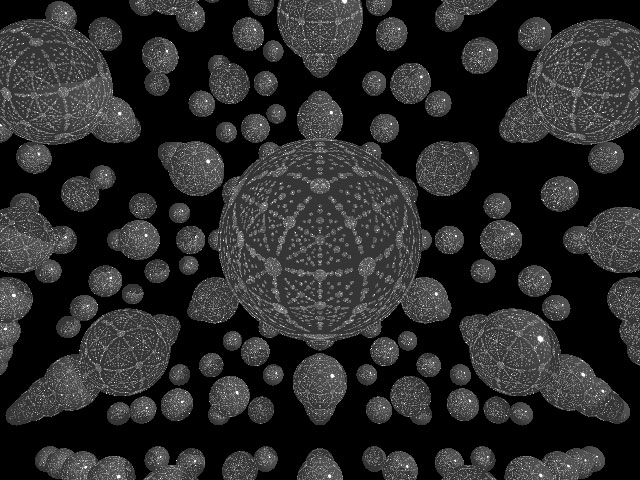
\includegraphics[width=10cm]{indrasNet.jpg}
\end{frame}

%%%%%%%%%%%%%%%%%%%%%%%%%%%%%%%%%%%%%%%%%%%%%%%%%%%%%%%%%%%%%
\begin{frame}
\frametitle{Example}

$C = \Vect_{G}$ for a finite group $G$.

\pause
$e$: trivial algebra $\kk_e$
\;\;\;
$\amod{e}(C) \simeq C_C$
\\
\pause
$f$: the group algebra $\kk[G] = \bigoplus \kk_g$
\;\;\;
$\amod{f}(C) \simeq \Vect$\\
(right action on $\Vect$ = forget $G$-grading)

\end{frame}

%%%%%%%%%%%%%%%%%%%%%%%%%%%%%%%%%%%%%%%%%%%%%%%%%%%%%%%%%%%%%
\begin{frame}
\frametitle{Example}

Next we study the functor categories.
Clearly the $C$-endofunctors of $C_C$ is $C$ itself.
\\
\pause
For $\amod{f}(C)$,
an endofunctor is given by some $m \in \bimod{f}{f}(C)$;
write $m = \bigoplus m_g$.
\pause
The right $f$-action on $m$ makes all the $m_g$ isomorphic
in a coherent manner.
\pause
For $h \in G$, conjugation (left action by $h$ and right action
by $h^\inv$) gives an action of $G$ on $m_e$;
determines $m$ completely.

\pause
Thus, $\ModA{C}(f,f) \simeq \bimod{f}{f}(C) \simeq \Rep(G)$.

\pause
(One can also check that $C$-module structure on
$m: \Vect \to \Vect$
amounts to $G$-action on $m(\kk)$.)

Thus we have:
\[
\ModA{\Vect_G} \simeq \ModA{\Rep(G)}
\]

\end{frame}

%%%%%%%%%%%%%%%%%%%%%%%%%%%%%%%%%%%%%%%%%%%%%%%%%%%%%%%%%%%%%
\begin{frame}
\frametitle{Example}

For functor categories between them, we see that
\[
\ModA{C}(e,f) \simeq \bimod{f}{e}(C) \simeq \amod{f}(C)
\simeq \Vect
\]
\[
\ModA{C}(f,e) \simeq \bimod{e}{f}(C) \simeq \moda{f}(C)
\simeq \Vect
\]

\pause
Note for $G = \ZZ/2$,
$\Vect_{\ZZ/2} \simeq \Rep(\ZZ/2)$,
don't see difference in endomorphism categories.

\pause
Of course, there are many other objects in $\ModA{C}$,
e.g. for a subgroup $H \subseteq G$,
have group algebra $\kk[H]$.
%which we denote by $h$ as an object in $C$.
%The category of modules $\amod{h}(C)$
%is simply the direct sum $\bigoplus_{H \backslash G} \Vect$,
%as the components $m_g$ of an $h$-module
%must be the same within each $H$-orbit.
%The endomorphism category seems a lot more complicated.
%\end{example}

\end{frame}

%%%%%%%%%%%%%%%%%%%%%%%%%%%%%%%%%%%%%%%%%%%%%%%%%%%%%%%%%%%%%
\begin{frame}

\begin{center}
\Huge End!
\end{center}

\end{frame}

%%%%%%%%%%%%%%%%%%%%%%%%%%%%%%%%%%%%%%%%%%%%%%%%%%%%%%%%%%%%%
\begin{frame}
\begin{thebibliography}{1}

\bibitem{DRfusion} Douglas, Christopher L., and David J. Reutter. ``Fusion
2-categories and a state-sum invariant for 4-manifolds.'' arXiv preprint arXiv:1812.11933 (2018).

\bibitem{Ostrik} Ostrik, Victor. ``Module categories, weak Hopf algebras and
modular invariants.'' Transformation groups 8, no. 2 (2003): 177-206.

\bibitem{DSPSa} C. L. Douglas, C. Schommer-Pries, and N. Snyder. The balanced tensor product of module
categories. Kyoto J. Math., 2017. arXiv:1406.4204.

\bibitem{DSPSb} C. L. Douglas, C. Schommer-Pries, and N. Snyder. Dualizable tensor categories. Mem. Amer.
Math. Soc., 2017. arXiv:1312.7188.

\bibitem{EGNO} P. Etingof, S. Gelaki, D. Nikshych, and V. Ostrik. Tensor Categories. American Mathematical
Society, 2015. Available online at http://www.math.mit.edu/~etingof/egnobookfinal.pdf.

\end{thebibliography}
\end{frame}


\end{document}


